%%%%%%%%%%%%%%%%%%%%%%%%%%%%%%%%%%%%%%%%%
% Short Sectioned Assignment
% LaTeX Template
% Version 1.0 (5/5/12)
%
% This template has been downloaded from:
% http://www.LaTeXTemplates.com
%
% Original author:
% Frits Wenneker (http://www.howtotex.com)
%
% License:
% CC BY-NC-SA 3.0 (http://creativecommons.org/licenses/by-nc-sa/3.0/)
%
%%%%%%%%%%%%%%%%%%%%%%%%%%%%%%%%%%%%%%%%%

%----------------------------------------------------------------------------------------
%	PACKAGES AND OTHER DOCUMENT CONFIGURATIONS
%----------------------------------------------------------------------------------------

\documentclass[letterpaper, fontsize=11pt]{scrartcl} % A4 paper and 11pt font size

\usepackage[T1]{fontenc} % Use 8-bit encoding that has 256 glyphs
\usepackage{fourier} % Use the Adobe Utopia font for the document - comment this line to return to the LaTeX default
\usepackage[english]{babel} % English language/hyphenation
\usepackage{amsmath,amsfonts,amsthm} % Math packages

\usepackage{lipsum} % Used for inserting dummy 'Lorem ipsum' text into the template
\usepackage[margin=1in]{geometry} %set margins -TA
\usepackage{sectsty} % Allows customizing section commands
\allsectionsfont{\centering \normalfont\scshape} % Make all sections centered, the default font and small caps
\usepackage{enumitem}
\usepackage{fancyhdr} % Custom headers and footers
\usepackage{graphicx}
\usepackage{float}

\usepackage{graphicx} % Required to insert images
\usepackage{multicol}
\usepackage{enumitem}
\usepackage{amssymb}
\usepackage{bm}
\usepackage{verbatim}
\usepackage{hyperref}
\usepackage{color}


\pagestyle{fancyplain} % Makes all pages in the document conform to the custom headers and footers
\fancyhead{} % No page header - if you want one, create it in the same way as the footers below
\fancyfoot[L]{\textit{CME 102 Winter '17-'18}} % Empty left footer
\fancyfoot[C]{} % Empty center footer
\fancyfoot[R]{Tim Anderson} % Page numbering for right footer
\renewcommand{\headrulewidth}{0pt} % Remove header underlines
\renewcommand{\footrulewidth}{0pt} % Remove footer underlines
\setlength{\headheight}{14pt} % Customize the height of the header

\numberwithin{equation}{section} % Number equations within sections (i.e. 1.1, 1.2, 2.1, 2.2 instead of 1, 2, 3, 4)
\numberwithin{figure}{section} % Number figures within sections (i.e. 1.1, 1.2, 2.1, 2.2 instead of 1, 2, 3, 4)
\numberwithin{table}{section} % Number tables within sections (i.e. 1.1, 1.2, 2.1, 2.2 instead of 1, 2, 3, 4)

\setlength\parindent{0pt} % Removes all indentation from paragraphs - comment this line for an assignment with lots of text
\begin{document}

%----------------------------------------------------------------------------------------
%	TITLE SECTION
%----------------------------------------------------------------------------------------

\newcommand{\horrule}[1]{\rule{\linewidth}{#1}} % Create horizontal rule command with 1 argument of height

%---------------------------------------------------------------------------------------a-
%	PROBLEM 1
%----------------------------------------------------------------------------------------

\section*{Final Review Problems}
\par If not otherwise specified, solve the following problems. If initial conditions are given, solve for all constants of integration. It is okay to leave answers in implicit form or with unsolved integrals. 

\begin{enumerate}

\item \textbf{Direction fields and Equilibrium solutions:} \par Identify the equilibrium solutions and state their type.
\begin{enumerate}

\item For the following figure:
\begin{figure}[h]
\centering 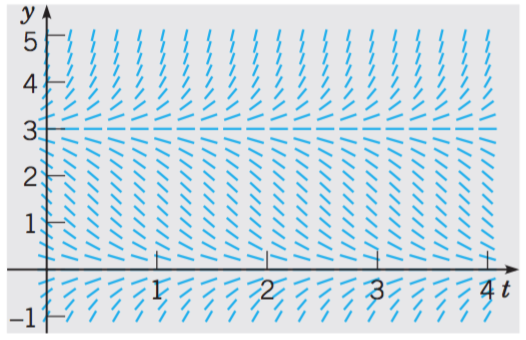
\includegraphics[width = 0.4\columnwidth]{finalReview1.png}
\end{figure}

\item  $y' = y(y-2)^2$

\item $y' = y(y - 3)(y-x)$

\end{enumerate}

\item \textbf{Solution verification:} Verify the solution to the following ODEs. 
\begin{enumerate}

% T&P equation 3.32
\item $x^2y''  + 2xy'  + y = \ln(x) + 3x + 1,\quad y = \ln(x) + x$

% T&P example 3.5
\item $(y'')^3 + (y')^2 - y - 3x^2 -  = 0, \quad y = x^2$

% T&P example 3.52
\item $y' = (x+y)^2,\quad y = \tan(x) - x$
\end{enumerate}

\item \textbf{Separation of variables:} Solve the following ODEs using separation of variables. 
\begin{enumerate}

\item $y' + y^2 \sin(x) = 0$ 

\item $y' =2+2x+2y^2 + 2xy^2, \quad y(0) = 0$

\item $y' =\frac{ty(4-y)}{1+t}$

\end{enumerate}

\item \textbf{Existence and uniqueness:} Give the interval for existence and interval for uniqueness of the solution. 
\begin{enumerate}

\item $\sin(2x)dx+\cos(3y)dy=0, \quad y(\pi/2) = \pi/3$

\item $y^2(1 - x^2)^{1/2}dy = \sin^{-1} (x) dx, \quad y(0) = 1$

\end{enumerate}

% First order and Bernoulli equation
\item \textbf{Linear first order ODEs:} Solve the following.
\begin{enumerate}

% B&D 2.1 example #3
\item $y' -2y = 4-t$

%B&D 2.1 #18
\item $ty' + 2y = \sin(t),\quad y(\pi/2) = 0$

\item $ty' + (t+1)y = t,\quad y(\ln(2)) = 1$

\end{enumerate}


% B&P 7.5 example 2 
\item \textbf{Eigenvector solution to ODEs:} Solve the following using an eigenvalue/vector system.

\[
\vec x' = \left[ \begin{array}{cc} 1 & 1 \\ 4 &1 \end{array} \right] \vec x
\]

% From: http://users.math.msu.edu/users/gnagy/teaching/13-fall/mth340/L09-340.pdf
\item \textbf{Nonlinear second order ODEs:} Solve the following. 
\begin{enumerate}

\item $y''  = -2t(y')^2, \quad y(0) = 2, \quad y'(0) = -1$

\item $y'' = 2y y'$

\end{enumerate}


\item \textbf{Second order linear ODEs:} Solve the following. Clearly state the method you are using and why.
\begin{enumerate}

% B&P 3.5 #28
\item $(x-1)y'' -xy' +y=5, \quad x>1,\quad  y_1(x)=x$
\par \textit{Hint 1:} The solution of $y'' = \frac{x^2 - 2x + 2}{x^2 - x}y'$ is $y = c_1\frac{e^x}{x} + c_2$
\par \textit{Hint 2:} $\int \frac{x}{e^x(x - 1)^2}dx = -\frac{e^{-x}}{x-1}$


\item $y'' -6y'+9y=e^{3t} +6$

\item $y'' -2y' +y=te^t +4,\quad y(0) = 1,\quad y'(0) = 1$

% B&P 3.6 #17
\item $x^2y'' -3xy' +4y=x^2 \ln(x)$

% B&P 3.6 #15
\item $ty'' -(1+t)y' +y=t^2e^{2t}, \quad t>0, \quad y_1 = t+1$
\par \textit{Hint:} the solution of $y'' = \frac{x^2+1}{x^2+t}y'$ is $y = c_1\frac{e^t}{t+1} + c_2$

\end{enumerate}


\item \textbf{Mass-spring system:} Consider the equation of motion for a mass-spring system:
\[ mx'' + \beta x' + k x = f(t) \]
For the following values of $m$, $\beta$, and $k$ and form of $f(t)$, state if the homogeneous solution is over-damped, critically damped, If the motion is forced, state whether we will have beats, resonance, or neither, and why.
\begin{enumerate}

\item $m = 1$, $\beta = 5$, $k = 2$, $f(x) = 0$

\item $m = 2$, $\beta = 0$, $k = \frac{1}{2}$, $f(t) = \sin(0.49t)$

\item $m = 2$, $\beta = 8$, $k = 8$, $f(x) = 0$

\item $m = 3$, $\beta = 0$, $k = \frac{1}{3}$, $f(t) = \sin(t/3)$

\item $m = 5$, $\beta = 2$, $k = 1$, $f(t) = \sin(2t/5)$

\end{enumerate}


\item \textbf{Laplace transform:} Solve the following using a Laplace transform
\begin{enumerate}

\item $y'' +2y' +2y=\cos(t)+\delta(t-\pi/2),\quad y(0) = y'(0) = 0$

\item $y'' + 4y' + 4y = te^{-2t},\quad y(0) = 0, \quad y'(0) = 1$

\end{enumerate}

\item \textbf{Circuits} Derive the system of differential equations for this circuit.

\begin{figure}[h]
\centering 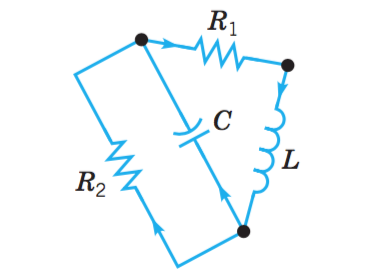
\includegraphics[width = 0.4\columnwidth]{finalReview2.png}
\end{figure}
How would you solve the system for this circuit? 

%\item \textbf{Power series:} Solve the following using a power series and give the recurrence relation. Write out your solution up to fifth order. Clearly state why you cannot use another method to solve the system.
%\begin{enumerate}
%
%% B&P 5.3 #16
%\item $(2+x^2)y'' -xy' +4y=0, \quad y(0) = -1, \quad y'(0) = 3$
%
%% B&P 5.3 17
%\item $y'' + xy' + 2y = 0$
%
%\end{enumerate}

\item \textbf{Direct method:} Consider the ODE
\[ y'' + x^2y = e^{-x}\]
Write out the direct method system of equations for the following boundary conditions for this ODE with $N=5$ nodes.
\begin{enumerate}

\item $y(0) = 0, \quad y(4) = 5$

\item $y(0) = 0, \quad 4y'(2) +  3y(2)= 5$

\end{enumerate}

\item \textbf{Numerical methods:} Write a short piece of MATLAB code to solve the following using backward Euler for $1 \leq t \leq 10$ with $h = 0.01$.
\[ y' + 5ty = \sin(t), \quad y(1) = 10\]

\end{enumerate}

%----------------------------------------------------------------------------------------

\end{document}